\documentclass[12pt]{article}

\usepackage[left=1in,top=1in,right=1in,bottom=1in]{geometry}
\usepackage{graphicx} % Required for the inclusion of images
\graphicspath{{../img/proposal/}}
\usepackage{float}
\usepackage{titlesec}
\setlength\parindent{24pt} %space for indentation
%\font\regfont=cmr12 at 13pt

% The title of your proposal should be informative, and must not exceed two printed lines. Please use mixed case instead of all upper case.
\title{\vspace{-2em} \Large \textbf{Correcting Keck/NIRC2's Systematic Errors \\ Using Linear SVMs}}
\author{Justin Kang}
\date{\vspace{-0.75em} \today}

\begin{document}
\maketitle


\vspace{-2em}
\section*{Abstract}
% Write a concise abstract describing the proposed investigation, including the main science goals and the justification for requesting observations or funding from HST. The abstract must be written in standard ASCII and should be no longer than 20 lines of 85 characters of text. This limit is enforced by APT.
\noindent Keck/NIRC2 uses AO to produce the highest-resolution ground-based images and spectroscopy in the 1-5 micrometer range. It is one of the best instruments for planet discovery and characterization, with 44 papers published just this year that have used it. However, there are several systematic errors that reduce its effectiveness and usability. Examples of these are read errors mirrored across the image quadrants, and the noisier lower-left quadrant. The current method of dealing with this noise is using a three-point dither pattern to reduce the effects of the bad quadrant and instrumental noise levels.\\\\ 
We propose to instead create a model of these errors. By doing so, we can then attempt to eliminate the bad quadrant, allowing for more usable image space, and also improve the deepness of the images by removing instrumental noise in all quadrants. One possiblity is training a linear support vector machine and using it to classify sources as either real or noise. Linear classifiers are compact, fast to train, fast to execute, and can be trained on large amounts of data, making them an ideal tool for this application. Furthermore the KOA database makes readily available large amounts of both training and testing data. Thus by successfully modeling and eliminating this noise, we can improve one of the best ground-based instruments for future use.


\newpage
\section*{Scientific Justification}
% This section should present a balanced discussion of background information, the program’s goals, its significance to astronomy in general, and its importance for the specific sub-field of astronomy it addresses. 
% AR Proposals should describe how the project improves upon or adds to the previous use of the data.
% Calibration Proposals should describe what science will be enabled by the successful completion of the program, and how the currently supported core capabilities, their calibrations, and the existing pipeline or data reduction software are insufficient to meet the requirements of this type of science.
\subsection*{Direct Imaging} % ~1 page
% https://en.wikipedia.org/wiki/Methods_of_detecting_exoplanets#Direct_imaging
% It is easier to obtain images when the star system is relatively near to the Sun, and when the planet is especially large (considerably larger than Jupiter), widely separated from its parent star, and hot so that it emits intense infrared radiation; images have then been made in the infrared, where the planet is brighter than it is at visible wavelengths. Coronagraphs are used to block light from the star, while leaving the planet visible. Direct imaging of an Earth-like exoplanet requires extreme optothermal stability.[48] During the accretion phase of planetary formation, the star-planet contrast may be even better in H alpha than it is in infrared – an H alpha survey is currently underway.[49]
% good at getting planets distant from stars
% Direct imaging can be used to accurately measure the planet's orbit around the star. Unlike the majority of other methods, direct imaging works better with planets with face-on orbits rather than edge-on orbits, as a planet in a face-on orbit is observable during the entirety of the planet's orbit, while planets with edge-on orbits are most easily observable during their period of largest apparent separation from the parent star.

\subsection*{Keck/NIRC2} % ~1 page
% https://en.wikipedia.org/wiki/W._M._Keck_Observatory#Instruments
% https://www2.keck.hawaii.edu/inst/nirc2/
% https://www2.keck.hawaii.edu/inst/nirc2/ObserversManual.html
% The second generation Near Infrared Camera works with the Keck Adaptive Optics system to produce the highest-resolution ground-based images and spectroscopy in the 1–5 micrometers (µm) range. Typical programs include mapping surface features on Solar System bodies, searching for planets around other stars, and analyzing the morphology of remote galaxies.
% The first multiplanet system, announced on 13 November 2008, was imaged in 2007, using telescopes at both the Keck Observatory and Gemini Observatory. Three planets were directly observed orbiting HR 8799, whose masses are approximately ten, ten, and seven times that of Jupiter
% A 3-pt dither pattern in the detector coordinate system. A bxy3 is basically a bxy5, but with the the lower left and central positions omitted. Due to elevated noise in the lower left quadrant, this has become the dither pattern of choice for many observing programs.
% GPI = 1020 nm - 2190 nm

\newpage
\subsection*{Proposed Program} % ~1 page
% https://en.wikipedia.org/wiki/Support_vector_machine
% https://en.wikipedia.org/wiki/Viola–Jones_object_detection_framework
% Given a set of training examples, each marked as belonging to one or the other of two categories, an SVM training algorithm builds a model that assigns new examples to one category or the other, making it a non-probabilistic binary linear classifier (although methods such as Platt scaling exist to use SVM in a probabilistic classification setting). 
% An SVM model is a representation of the examples as points in space, mapped so that the examples of the separate categories are divided by a clear gap that is as wide as possible. New examples are then mapped into that same space and predicted to belong to a category based on which side of the gap they fall.
% The Viola–Jones object detection framework is the first object detection framework to provide competitive object detection rates in real-time proposed in 2001 by Paul Viola and Michael Jones. Although it can be trained to detect a variety of object classes, it was motivated primarily by the problem of face detection.


\newpage
\begin{figure}[H]
\centering
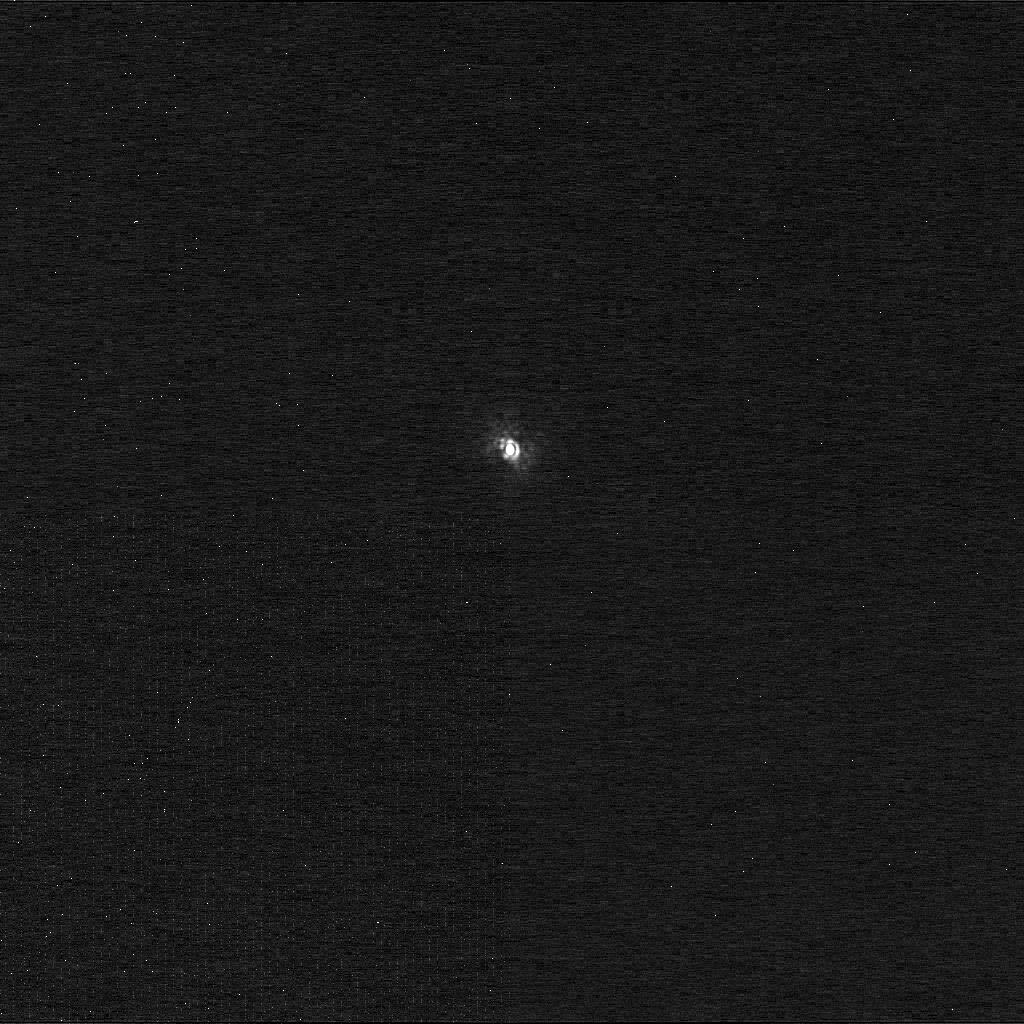
\includegraphics[width=0.45\textwidth]{image.jpg}

\includegraphics[width=0.45\textwidth]{corner.jpg}
\vspace{-0.75em}
\caption{blah blah blah}
\end{figure}
\begin{figure}[H]
\centering
% 4th root versions
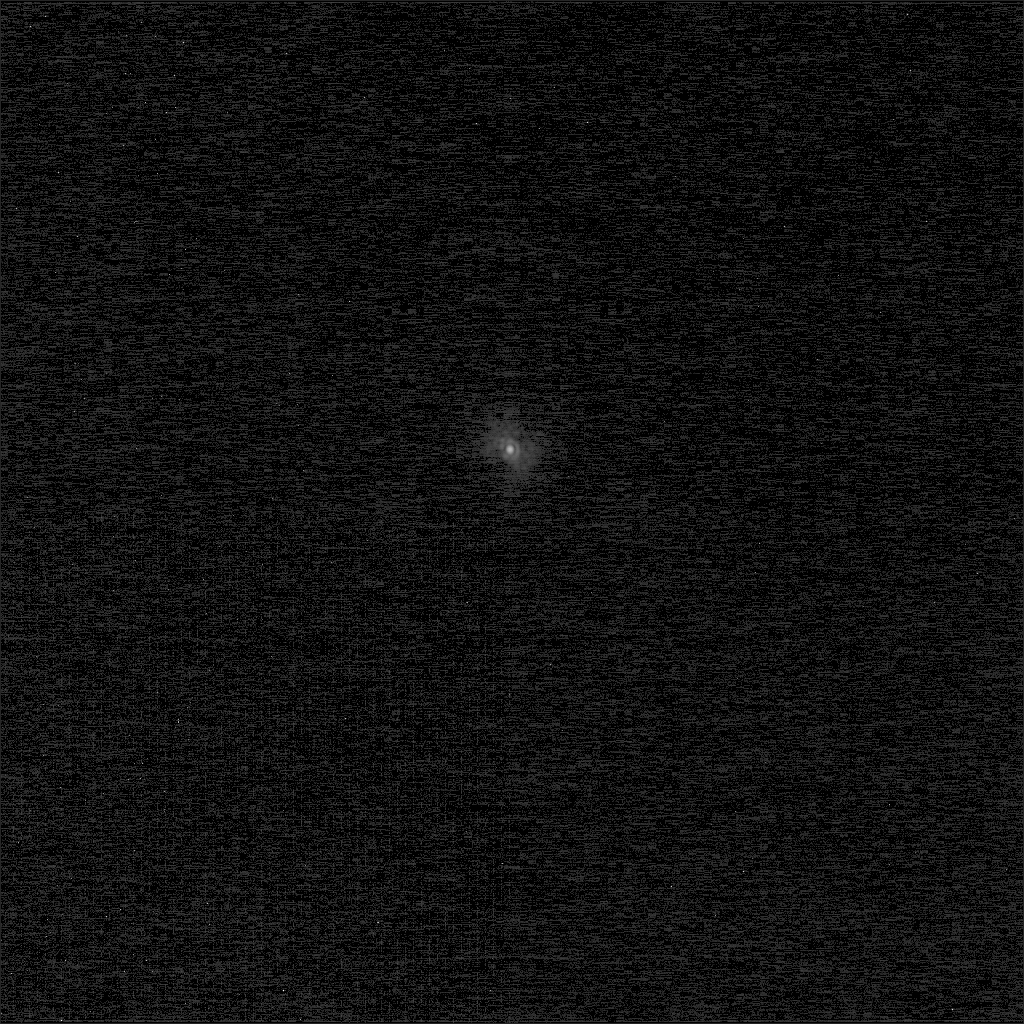
\includegraphics[width=0.45\textwidth]{image_root.png}

\includegraphics[width=0.45\textwidth]{corner_root.png}
\vspace{-0.75em}
\caption{blah blah blah}
\end{figure}


\newpage
\section*{Analysis Plan} % ~1 page
% All AR Proposals should provide a detailed data analysis plan and describe the datasets that will be analyzed. Proposers should complete the information required in the APT dataset table (see Section 8.14): the number of datasets (not pointings) per instrument needed to carry out the research and the type of data retrieval (ftp, DVD, or disk: see the HST Archive Data Retrieval Options for a description of the available options). Proposers must provide a schedule indicating the timescale for the data request(s), for example all datasets at once, or 1/12th of the datasets per month. Inclusion of a complete target list is not required.
% Calibration Proposals should discuss what documentation, and data products and/or software will be made available to STScI to support future observing programs. Proposers should explain how their programs complement ongoing calibration efforts by the instrument groups. They should contact the relevant groups to ensure that efforts are not duplicated.


\newpage
\section*{Management Plan} % ~1 page
% Provide a concise, but complete, management plan. This plan will be used by the review panels to assess the likely scale of the proposed research program. Proposers should include a schedule of the work required to achieve the scientific goals of the program, a description of the roles of the PI, Co-Is, postdocs, and students who will perform the analysis, and a plan to disseminate the results to the community.


\newpage
\bibliographystyle{ieeetr}
\bibliography{mybib}

\end{document}